\documentclass[11pt,a4paper]{article}
\usepackage{bbm,amsthm,amsfonts,amssymb,amsmath,nicefrac,latexsym,epic,eepic}
\usepackage{marvosym,graphicx,fancyhdr,bbm,psfrag}
\usepackage{hyperref}
\usepackage[dvips]{color}
\usepackage[rflt]{floatflt}
\usepackage{colortbl}
\definecolor{Grey}{rgb}{0.3,0.3,0.3}
\definecolor{Red}{rgb}{1.0,0.0,0.0}
\usepackage{typearea}
\areaset{156mm}{235mm}
%\setlength{\parskip}{5pt plus 2pt minus 1pt}
\setlength{\parindent}{0pt}

% use \M for matrices and \V for vectors in math mode
\newcommand{\M}[1]{\mathbf{#1}}
\newcommand{\V}[1]{\mathbf{#1}}
\newcommand{\norm}[1]{\left | \left | #1 \right | \right |}
\newcommand{\RR}{\mathbbm{R}}        % set of real numbers


\renewcommand\floatpagefraction{0.8}
\renewcommand\topfraction{1}
\renewcommand\bottomfraction{0.9}
\renewcommand\textfraction{0.0}
%\def\dbltopfraction{1.0}
%\def\bottomfraction{1.0}
%\def\dblfloatpagefraction{0.8}

\hypersetup{
    colorlinks=true,
    linkcolor=Red,
    urlcolor=blue,
    citecolor=black,
}

\makeatletter
\renewenvironment{thebibliography}[1]
     {\section*{\refname}%
      \@mkboth{\MakeUppercase\refname}{\MakeUppercase\refname}%
	 \parsep0mm
	 \itemsep0mm
	 %\labelsep0mm
	 %\itemindent0mm
      \list{\@biblabel{\@arabic\c@enumiv}}%
           {\settowidth\labelwidth{\@biblabel{#1}}%
            \leftmargin\labelwidth
            \advance\leftmargin\labelsep
            \@openbib@code
            \usecounter{enumiv}%
            \let\p@enumiv\@empty
            \renewcommand\theenumiv{\@arabic\c@enumiv}}%
      \sloppy
      \clubpenalty4000
      \@clubpenalty \clubpenalty
      \widowpenalty4000%
      \sfcode`\.\@m}
     {\def\@noitemerr
       {\@latex@warning{Empty `thebibliography' environment}}%
      \endlist}
\renewcommand\newblock{\hskip .11em\@plus.33em\@minus.07em}
\let\@openbib@code\@empty
\makeatother

\usepackage{hyperref}

\begin{document}

\title{\Large\bf Kimera - an open source library for metric-semantic Visual-Inertial Simultaneous Localization And Mapping\footnote{This paper has been written as part of the seminar 3D mapping and geometry processing for underwater and aerospace applications in Winter 2023/24}}

\author{Ken Schlesiger\\
  Informatics XVII \\
  University of Würzburg\\
  Am Hubland, D-97074 Würzburg, Germany\\
{\small \texttt{ken.schlesiger@stud-mail.uni-wuerzburg.de}}}

\date{}

\maketitle

\newpage
\begin{abstract}
    
Kimera is a modular and accurate library for real-time Visual inertial odometry, pose graph optimisation, 3D-Mesh construction and semantic segmentation.
It is able to be run in a performance constraint environment without the use of a GPU for processing. 


Kimera is meant to provide a flexible and extensible basis for future research in the fields of semantic segmentation, Visual inertial odometry and 3D mesh generation.
\end{abstract}

\section{Introduction}\label{Sec:Intro}
In recent years the fields of computer vision, robotics and autonomous systems have undergone remarkable advancements. The ability to quickly estimate the 3D geometry of a scene and understand its contents enable such complicated tasks as the interaction of robots with their surroundings or self driving cars. 
These processes require real-time and accurate spatial perception for safe navigation and effective interaction with the environment.
Kimera \cite{rosinol2020kimera} is an open-source Library designed for metric-semantic Visual-Inertial Simultaneous Localization And Mapping (SLAM), which is meant as a basis for further research and development of such systems. The Kimera Library offers state of the art approaches to Visual inertial Odometry, pose graph optimisation, mesh reconstruction, and 3D semantic segmentation.
The Library is designed to run in real time on only a CPU instead of a GPU, as is the used by most other 3D mapping libraries. 
Kimera achieves this by fusing the fields of 3D-geometric reconstruction of an area with semantic segmentation, which have traditionally been seen as separate areas of research. 
Kimera goes beyond existing visual and visual-inertial SLAM libraries by not only providing fast and accurate state estimates, but also allowing for real time mesh reconstruction and semantic labeling.
The Library is comprised of four main components: a visual inertial odometry module, a pose graph optimisation module, a lightweight 3D mesh generation module and 3D metric-semantic reconstruction module.

Unlike many existing libraries, which use RGB-D cameras or LiDAR, Kimera focuses on visual and inertial sensing using a pair of stereo cameras to broaden the range of environments that can be reliably mapped. 

For further details, the complete documentation and supplementary material can be found on the Kimera GitHub repository: \url{https://github.com/MIT-SPARK/Kimera}\\ A demonstration video is available on YouTube: \url{https://www.youtube.com/watch?v=-5XxXRABXJ}
\section{Background} \label{Sec:background}
This section is mainly split into two parts: \emph{(i)} A short overview over similar Libraries before Kimera, \emph{(ii)} a short overview over similar libraries since the release of Kimera.
\subsection*{\emph{(i)} Historical overview over similar Libraries}
Before the release of Kimera several Libraries with similar functionality have been released. 
Many of these libraries do however differ significantly from Kimera.
The approaches these libraries use are usually either lidar or rgb-d camera based, simpler, or unable to perform in real time. 
Simpler approaches include Kalman-Filter based approaches, for example MSCKF based approaches like 
\cite{MSCKF} or \cite{sun2018robust}. 
A library that combines many of these approaches is VINS-Fusion~\cite{qin2019b}, which allows for state estimation with both Cameras and lidars, as well as GPS data alongside many other sensors in a optimization based state estimator. 
According to \cite{ORBSLAM3} Kimera and VINS-Fusion perform similarly.
Another library with the intention of providing a basis for VIO research is openVINS~\cite{Geneva2020ICRA}, it focuses on the previously mentioned MSCKF as the core of its library. 

\subsection*{\emph{(ii)} Overview over similar Libraries since the release of Kimera}
Since the release of Kimera in 2019 several libraries have been released that implement some of the features that Kimera supports.
The most notable of these libraries is ORB-SLAM3~\cite{ORBSLAM3}, which is a library for real time visual slam using monocular, stereo and RGB-D cameras. 
While the general implementation of Orb-SLSM3 is distinct from that of Kimera, it is notable that is able to consider all measured states while Kimera only considers those in a certain time frame. 
Orb-SLSM3 is also able to create multiple local meshes and merge them to improve its performance.
It however does not build a semantic mesh. 
In a comparison between Kimera an Orb-SLAM3 the authors claim that Orb-SLAM3 is three two four times more accurate than Kimera and VINS-Fusion on the EuRoC dataset. 
Another library that outperforms Kimera is OKVIS2 \cite{leutenegger2022okvis2}, which leverages old marginalized states in its factor graph as well as a convolutional neural network to remove dynamic objects and significantly outperforms Kimera in pose estimation. 

It is notable that Kimera doesn't produce its own semantic labels. 
A library which achieves this is \cite{murez2020atlas}.
This approach to semantic segmentation uses back projected 2D semantic labels generated using a 2D Convolutional neural network, as well as a 3D CNN to predict a 3D model. 

It is notable that none of the libraries, released before or after Kimera include all of the features that Kimera implements,
mainly both semantic segmentation as well as 3D metric semantic annotation.



 
\section{Kimera} \label{Sec:kimera}
\subsection{Structure}
Kimera is build from four independent modules: 
\begin{itemize}
    \item \textbf{Kimera-VIO:} A GTSAM \cite{gtsam} based visual inertial odometry Module. Kimera-VIO allows for IMU-rate state estimation. 
    \item \textbf{Kimera-RPGO} A pose graph optimizer with modern outlier rejection.
    \item \textbf{Kimera-Mesher} A module that efficiently generates both per frame and multi frame regularized 3D meshes. 
    \item \textbf{Kimera-Semantics:} A module that builds a more accurate and volumetric 3D mesh than Kimera-Mesher and semantically annotates the mesh using 3D semantic segmentation. 
\end{itemize}
Each module is able to perform independent from the other modules. 
This allows the user to replace or modify the Modules as they see fit swell as run each module on their own if only a subset of the functionality is required.
Due to Kimeras Lightweight design, being able to run on only a CPU, each module is not only able to run  offline using a previously generated dataset, but also able to run online on a real time system using the Robot operating system (ROS).

\subsection{Kimera-VIO}
\ref{pre:on-manifold} to \ref{Sec:Lucas-Kanade} are meant to explain important topics to Kimera-VIO.
\ref{Sec:K-VIO overview} explains the inner workings of Kimera-VIO.

\subsubsection{On-manifold Preintegration} \label{pre:on-manifold}
In theory the IMU measurements can be integrated between time $t_i$ and $t_j$.
Problems do however arise in the context of optimisation based state estimation. 
Here the state of the system at time $t_i$ is unknown and changes as more data points become available during successive steps of optimisation.
T. Lupton and S. Sukkarieh \cite{preint_lupton} propose the use of pseudo measurements independent from the instal conditions which only describe the motion between measurements.
Forster \textit{et al.} \cite{Forster_2017} improve on this by providing a more mathematically rigorous approach that avoids the problem of singularities caused by the use of euler-angles. 
Their approach also generates a factor graph allowing for the use of incremental smoothing algorithms. 
They also use a structureless model which reduces the computational load while retaining accuracy.
todo rewrite section

\subsubsection{Shi-Tomashi Corners} \label{Sec:Shi-Tomashi}
Corners denote areas where a slight shift in location leads to a large change in pixel value. 
The Shi-Tomashi~\cite{Shi_tomasi} algorithm is a modification of the Harris corner detection algorithm. 
It is comprised of three steps: \emph{(i)} identification of which areas lead to large shifts in pixel value, \emph{(ii)} calculate the \textit{"R"} score and \emph{(iii)} select the important corners.
\subsubsection*{\emph{(i)} identification of areas of interest} 

This is done with the following formula\footnote{In actuality the Taylor-series expansion of E(u,v) is used as its performance requirements are lower.}:
\begin{align}
    E(u,v) = \sum_{x} \sum_y w(x,y) [I(x+u,y+v)- I(x,y)]^2  
\end{align}
x and y denote the position of a pixel, while u and v denote the amount of displacement of a pixel.
w(x,y) is a function dependent on the shape of the window that is being calculated. 
The functions $I(x+u,y+v)$ and $I(x,y)$ denote the Intensity of a pixel in an Image.
For example in a greyscale image this would be the brightness of a pixel.
Therefore the term $I(x+u,y+v)- I(x,y)$ describes the relative shift of the intensity between two pixels. For a corner this value would be very large.
\subsubsection*{\emph{(ii)} calculating the \textit{"R"} score} 

This is done with the following simple equation:
\begin{align}
   R = min(\lambda_1, \lambda_2) 
\end{align}
$\lambda_1$ and $\lambda_2$ are the Eigenvalues of the Taylor-series expansion of $E(u,v)$
\subsubsection*{\emph{(iii)} Corner selection} 
The selection of satiable corners is done by classifying all R values above a certain threshold as corners.

\subsubsection{Lucas-Kanade Tracker} \label{Sec:Lucas-Kanade}
The Lucas-Kanade tracker is a algorithm that tracks the positions of points in a video, that are moving due to camera movement or movement in the foreground.
The Lucas-Kanade tracker works on the assumption that the brightness between two frames in a Video-stream is relatively constant. 
Mathematically this assumption can be written as:
\begin{align} \label{eq:optical}
        I_x u + I_y w + I_t = 0 
    \end{align}
Where the 2D positional gradients are expressed by $I_x = \frac {\partial I} {\partial x}, I_y = \frac {\partial I} {\partial y}
$ and the temporal radian by $I_t = \frac {\partial I}{\partial t}$.
u and v denote the movement in the x and y directions respectively.

Equation~\ref{eq:optical} cannot be solved as it is underdetermined.
Therefore the movement is observed over multiple points $p_0$ - $p_n$.
This can be mathematically expressed as:
\begin{align} \label{eq:lk-solved}
    \begin{pmatrix}
        I_x(p_0) & I_y(p_0) \\  ... \\ I_x(p_n) & I_y(p_n)
    \end{pmatrix} 
    \begin{pmatrix}
       u \\ v
    \end{pmatrix} = 
    \begin{pmatrix}
        I_t(p_0) \\  ... \\ I_t(p_n) 
    \end{pmatrix} 
\end{align}
Noise in real data will render equation~\ref{eq:lk-solved} unsolvable as the system is overconstrained.
Therefore, instead of solving for u and v analytically the equivalent least squares problem needs to be solved to determine the camera movement.

\subsubsection{Smoothing Based State Estimation} \label{Pre:Smoothing}
In the field of VIO exist two main smoothing approaches, Fixed-Lag and full smoothing.
Full-smoothing based approaches smooth over all state-measurements, while Fixed-Lag smoothing marginalizes out all old states and therefore only considers those in a certain time frame.
The general Approach is otherwise similar: It begins with estimating the state in the relevant Time frame.
The optimisation is done by comparing the measured IMU and visual data with a state prediction by using a cost function. 
The goal of the optimisation is to minimize this cost function at all points in time to get a trajectory that best fits the measurements.

\subsubsection{Random sample consensus} \label{sec:RANSAC}
RANSAC is a method that randomly selects n points and fits a model through them.
Then the distances of each point to the model are determined. 
After that a score is calculated by counting the number of points which support this model.
This process is repeated several times or until all possible combinations of n points have been considered. 
The function with the largest highest score is then selected as the best fit.

\subsubsection{Overview} \label{Sec:K-VIO overview}
The Kimera visual inertial odometry (VIO) module outputs state estimates of the robot.
As input it requires both stereo camera frames and IMU data. 
While approaches based on filtering (e.g. Observationally constraint EKF, iterative EKF ) are used in Visual Inertial Odometry they tend to degrade in performance over time as they render themself inconsistent~\cite{Forster_2017}. 
Therefore Kimera employs Fixed-Lag smoothing (see sec.~\ref{Pre:Smoothing}) based state estimation in form of  a modified version of the On-Manifold Preintegration (see sec.~\ref{pre:on-manifold}) algorithm presented in \cite{Forster_2017} which computes a maximum a posteriori estimate in real time. 
This paper improves on the runtime constraints of usual VIO approaches by preintigrating the inertial measurements between keyframes into a single motion. 
This means that certain quantities will be computed between keyframes reducing the amount of variables that need to be optimized. 
Kimera expands on this to use both monocular and stereo cameras instead of only monocular cameras and also to allow both full lag and fixed lag smoothing, though fixed lag smoothing is used preferentially to limit the time the algorithm takes.

Kimera-VIO is split into two parts: \textit{(i)} The front-end and \textit{(ii)} the back-end. 
The front end is responsible for feature tracking, preintigration of measurements between keyframes, while the back-end is responsible for the state estimation using the fixed lag smoother. 
\subsubsection*{\textit{(i)} The Front-end}\label{para:geometric verification} 

The Kimera-VIO front-end is split between the IMU based front-end and the vision based front-end.
The IMU based front-end is processing IMU-data by performing the modified on-manifold preintegration to generate the relative measurements between two keyframes. 
The vision based front-end first detects Shi-Tomashi (see ~\ref{Sec:Shi-Tomashi}) corners. 
These corners are then tracked using the Lucas-Kannade Tracker \cite{lucas1981iterative} (see ~\ref{Sec:Lucas-Kanade}). 
Matches between the detected features in the left and right stereo images are then detected.  

Kimera performs this geometric verification on both monocular vision using 5-point RANSAC (see sec.~\ref{sec:RANSAC}) and stereo vision using 3-point RANSAC.
Kimera also offers the ability to verify the IMU data using mono and stereo verification using 2 and 1-point RANSAC respectively.

\subsubsection*{\textit{(ii)} The Back-end}
The VIO back-end uses the preintegrated IMU measurements and a structureless \footnote{In this context structureless means that the Positions of landmarks (tracked features) are ignored by the fixed lag smoother} visual model similar to \cite{Forster_2017} and adds them to a fixed lag smoother.
The fixed lag smoother is a factor graph. 
iSAM2 implemented in the GTSAM library is then used to solve the factor graph. 
iSAM2 is an incremental soothing technique which uses factor graphs to reduce the number of variables that full smoothing approaches inherently have to compute. 
After each iSAM2 computation produces the newly refined state estimates the 3D-positions of features tracked by the VIO front-end are determined.

This is done by the use of a direct linear transformation (DLT). 
DLT is a technique that leverages the geometry of the stereo camera to calculate the 3D position of the tracked features.
These features are then removed from the factor graph as they are not required for state estimation.

Degenerate points and outliers are then removed from the data to ensure better performance.
The last step of the VIO back-end algorithm is the marginalisation of all states that fall out of the VIO time horizon as these points will no longer be smoothed over.


\subsection{Kimera-Mesher}
Sec.\ref{pre:delaunay} is meant to explain important topics to Kimera-VIO.
Sec.\ref{Sec:K-Mesher overview} explains the inner workings of Kimera-VIO.
\subsubsection{Delaunay Triangulation} \label{pre:delaunay}
Delauny Triangulation is a method used for creating 2D-Meshes\footnote{These meshes can also be generated in higher dimensional spaces, however Kiemra only uses the 2D case.} over a set of points.
This is done by selecting ovals in such a manner that each oval contains exactly three points within its area.
Each point should also be on the edge of one of the ovals.
When these criteria are met all the points belonging to one oval are connected.
This process them forms a 2D-Mesh.

\subsubsection{Overview} \label{Sec:K-Mesher overview}
The Kimera-Mesher produces two kinds of 3D mesh: 
First per-frame mesh and second a multi-frame mesh.
The per-frame mesh is generated every frame from the stereo camera input, while the multi-frame mesh is generated from the per-frame mesh.
The per-frame mesh is generated from the points that Kimera-VIO front-end tracks in the current key frame. 
To generate the per-frame mesh first, these points are triangulated in 2D (see ~\ref{pre:delaunay}).
This triangulation is then projected onto the results of the Kimera-VIO back-end. This results in a 3D mesh. 
The multi-frame mesh is then constructed from the output of the per-frame mesh.
To achieve this Kimera-Mesher determines which edges and vertices of the per-frame mesh aren't jet contained in the multi frame mesh and adds them to it accordingly. 
The positions of all vertices are then updated with new position estimates produced by the Kimera-VIO back-end.
Next vertices that have fallen behind the VIO time horizon get removed. 
Finally when planar structures are detected, regularity factors are added to the multi frame mesh to improve mesh quality.

\subsection{Kimera-RPGO}

\subsubsection{Incremental Consistent Measurement Set Maximization} \label{pre:PCM}
Incremental Consistent Measurement Set Maximization is a  method of detecting loop closures in multi robot SLAM applications. 

It takes a set of putative loop closures as input and tries to filter out all pairwise inconsistent loop closures. 
This is done by finding pairs of measurements that support each other. 
A maximum subset of these consistent measurements is then selected as the proper trajectory.
This is efficiently solved by converting the problem into a Maximum Clique problem over a consistency graph. 
A Maximum Clique problem looks for the largest subset of vertices where all vertices have edges between them. 
A consistency graph is defined as a graph where each vertex represents a measurement and each edge denotes a consistency.
This consistency is determined by the use of a consistency metric, for example the Mahalanobis distance.
This is then represented via the use of a adjacency matrix.
The values in the matrix represent the values determined by the consistency metric. 
\subsubsection{The Gauß-Newton Method} \label{pre:Gauß-netwon}
Gauß-Newton is a method for solving non linear least square problems. 
As such it is an iterative optimisation technique that seeks to minimize the sum of squared differences between observed and predicted values.
This is achieved by linearising the model using a Jacobian and solving the linearised least squares problem at each iteration.
\subsubsection {Overview}
Kimera-RPGO is split into two parts: \textit{(i)} a loop closure detection algorithm and \textit{(ii)} a Pose Graph optimisation module that calculates a globally consistent pose.


\subsubsection*{\textit{(i)} Loop Closure Detection}
Loop Closure Detection denotes the detection of areas that the robot has previously visited.
This is done as errors in the estimated map and pose can accumulate over time resulting in an offset.
If loop closures are detected, these offsets can be corrected. 
Kimera-RPGO detects putative~\footnote{putative loop closures are candidates for loop closures.} loop closures by a bag-of-words representation using DBoW2~\cite{dbow2} . 
A bag of words representation is a set that usually contains a histogram which groups visual words together. 
A visual word is created by grouping similar visual features in the observed environment together.
If two of these bags of words are significantly similar a putative loop closure is detected. 

Kimera-RPGO then verifies loop closures using mono and stereo geometric verification similar to \ref{para:geometric verification}\textit{(i)}. This set can however still contain outliers, these may be caused by similar locations.
The remaining loop closures are then passed to the robust PGO-solver.

\subsubsection*{\textit{(ii)} Robust PGO-Solver} 
The Kimera-RPGO Pose graph optimizer uses a modified version of \textit{Consistent measurement Set Maximization}~\cite{PCM} (see \ref{pre:PCM}) (PCM). PCM has been modified to not only work on a single robot, but also in a real time (online) case.
PCM has been further modified to also check its output using 1.Odometry and 2.Comparing previous loop closures to the newly detected ones. 
In 1. outliers are detected by comparing odometry and PCM. 
If the PCM is an outlier it should differ from the odometry by a larger difference than that off measurement noise\footnote{Anomalous odometry outliers are filtered out through a Chi-squared test.}. After this the loop closures are compared to previous ones. 
Kimera-RPGO also differs in how it builds its adjacency Matrix $\M{A}$.
While PCM builds a new $\M{A}$ every time a loop closure is detected, Kimera-RPGO adds new rows and columns to its adjacency matrix each time a new loop closure is detected. This ensures the performance constraints needed for real time operation.
Finally the largest subset is determined using a maximum clique algorithm (see \ref{pre:PCM}) and the results are added to the pose graph after some optimisation using the Gauß-Newton method (see \ref{pre:Gauß-netwon}).

\subsection{Kimera-Semantics}
\subsubsection{Semi-Global Matching} \label{pre:semi-global matching}
Semi-global matching is a method used  to compute the correspondences between pixels in a pair of stereo images. 
This yields a disparity image between the two images. 
A disparity image is an image which describes the apparent motion\footnote{An example of apparent motion would be the perceived jump in the position of ones thumb when covering ones eye.} between images.
The disparity image is calculated by finding pixels with similar intensity in the stereo pair. 
However this does result in many erroneous matches for each pixel. 
To prevent this a regularisation factor is used which penalises jumps in the disparity between adjacent pixels.
\subsubsection{Truncated singed distance field} \label{pre:TSDF}
A signed distance field describes the distance of points in space to the nearest surface.
If the point is outside of the object its sing is positive.
If the point is inside the object the sing is negative. 
If the point is on the surface of a object, it is 0. 
In this context truncation means that we only consider points with a certain maximum distance and discard the rest. 
\subsubsection{Marching cubes} \label{pre:marching cubes} 
\begin{figure}
  \centering
  \includegraphics[width=80mm]{MarchingCubesEdit}
  \caption{The 15 basic shapes of marching cubes (source~\cite{marchingCubesImage})}\label{Fig:Marching cubes}  
\end{figure}
Marching cubes is a algorithm that approximates a 3D mesh from a voxel grid. 
A voxel grid is a list of values regularly spaced through the volume. 
Marching then "marches" a "cube" consisting of eight  points adjacent to each other.
A point is called active if the value of a corresponding voxel is above a certain threshold.
If one of these points is active, its connecting edges form a triangle. 
If not just one of these points is active, these shapes become more complex leading to $2^8$ different configurations with 15 unique cases\footnote{The missing cases are all symmetries of the 15 cases.} as seen in \ref{Fig:Marching cubes}.

Marching cubes loops over the voxel grid and creates the boxes filled with one of the $2^8$ shapes according to the values of the voxels.

\subsubsection{Overview}
Kimera semantics serves two main functions: \textit{(i)} Building an accurate 3D-Mesh and  \textit{(ii)} semantically annotating that mesh.
If no labels are provided, only the 3D-mesh will be build as semantic annotation is not possible.
The user of Kimera-Semantics has to provide their own labels as Kimera-Semantics dost generate the labels. 
According to a comment by one of the contributors when asked about appropriate models on the GitHub of Kimera-Semantics any "any that outputs semantic labels on a per-pixel basis will do".

Kimera-Semantics doesn't use the mesh created by Kimera-Mesher. 
This is due to higher level tasks requiring a more accurate 3D-mesh than those required by low level tasks like obstacle avoidance.
\subsubsection*{3D Mesh Generation and Annotation}
With 3D mesh generation an annotation is achieved in Kimera Semantics via the use of semi-global matching~\cite{SGM} (see \ref{pre:semi-global matching}) by leveraging information about the camera position and geometry and triangulating the corresponding 3D positions.
The provided labels are attached to the generated 3D-Point cloud. 
Voxblox is then used to create a TSDF (see \ref{pre:TSDF}) using grouped ray casting.
In voxbloxes grouped ray casting each point is mapped to the nearest voxel on the voxel grid. 
The mean of all positions is then taken and a ray cast to this mean. 
The probabilities of the labels are simultaneously generated by counting the occurrences of each label. 
While the ray travels through the voxel grid the probabilities of the labels are updated accordingly, by Bayesian updates. 
Finally the marching cubes algorithm is used to extract a 3D-mesh with the labels.

\subsection{Performance}
To allow the Kimera Modules to run independently Kimera uses four Threads. 
This is required due to the differing run time requirements of the different components.
The authors measured the preintegrating part to have a runtime of 40µs while the visual feature tracking takes a lot longer at an average of around 4.5 ms with a maximum of more than 60ms.
This allows the front-end to estimate the position at over 200Hz.
The VIO back-end runs slower at a mean runtime of 45ms, most of this time is consumed by solving the factor graphs at a runtime of 40ms. 
It is notable that the time for feature tracking at each frame is significantly shorter than the feature detection, stereo matching,
and geometric verification executed at each keyframe as seen in \ref{Fig:Timings}.
Kimera-Mesher generates the per-frame mesh at below 5ms and the multi-frame at below 15ms leading to a total run time of under 20ms.
Due to Kimera-RPGO and Kimera-Semantics usually not being time critical for real time systems, as they would be used for higher level tasks like path planning, they run on slower threads then Kimera-VIO and Kimera-Mesher which are necessary for vital processes like obstacle avoidance.
Kimera-RPGO has a measured runtime of less then 55ms.
The longest runtime is that of Kimera-Semantics at an average of 100ms at each keyframe. 
Kimera-VIO runs on the first two threads, with its front-end running on the first thread.
The second thread is shared by the Kimera-VIO back-end and Kimera-Mesher.
This is due to Kimera-Mesher using the calculated pose of the VIO back-end to update the positions of the vertices of the multi-frame mesh.
The third and fourth thread run Kimera-RPGO and Kimera-Semantics respectively. 

\subsection{Results}
The authors of Kimera tested the modules of Kimera independently from one another. 
All tests were done on either measured real world datasets or done in a simulator.
The authors of Kimera compared their VIO approach to 5 other open source VIO piplines: OKVIS, MSCKF, ROVIO, VINS-Mono, and SVO-GTSAM.
They tested these pipelines on 11 different datasets.
Among these approaches four (OKVIS, MSCKF, ROVIO, VINS-Mono) implement fixed lag smoothing. 
SVO-GTSAM allows for full-lag smoothing and VINS-LC for Loop closure detection. 
In fixed-lag smoothing Kimera showed the best performance on 8 out of the eleven datasets and being tied on one of the datasets. 
On the reaming two datasets Kimera measured second best.
In full smoothing Kimera outperformed GTSAM 6 times while being tied twice. 
It is also notable that GTSAM failed completely three times while Kimera was able to run all tests.
In PGO Kimera outperformed VINS-LC 9 out of 11 times. 
It is also notable that Kimera-VIO incurs a small drift of below 0.2 $\%$ on longer trajectories. 
The authors also measured the impact of the tunable parameter of Kimera-RPGO and found that it only impacts the performance of Kimera by a negligible amount when using PCM.
They measured a RMSE of 0.05 m at a $\alpha$ of 10 and a RMSE of 0.049 m at a $\alpha$ of 0.001, when using PCM. 
Without the use of PCM the error increases to a maximum of 1.59 m at a $\alpha$ of 0.001. 
To evaluate the performance of Kimera-Mesher testing on six sequences in the EuRoC V1 and V2 datasets was done. 
The performance of both the Multi-frame mesh as well as the global mesh was determined. 
The Multi-frame mesh hat a RMSE of 0.374 m and 0.530 m, while the error of the Global mesh was between 0.353 m and 0.480 m.
The Global Mesh outperformed the Multi-frame mesh in four out of the six tests, ranging from 12 \% to 24 \% lower RMSE.
In the cases where the multi-frame mesh was more accurate the difference was less than 3 \%.
The testing of Kimera-Semantics was done using a unity based simulator. 
The authors noticed small geometric and semantic errors with bundled raycasting, while dense stereo introduces notable errors, especially in texture-less areas like walls. 
Using ground truth depth and pose information provided by the simulator a semantic accuracy of 94.68 \% was achieved, with a geometric RMSE of 0.079 m.
The impact of the use of Kimera-Vio is mainly visible in the 3D mesh with its RMSE increasing to 0.131 m, while the semantic accuracy remains at 94.50 \%. 
The use of Dense stereo instead of ground truth depth sees both measures worsen to a semantic accuracy of 80.74 \% and a RMSE of 0.215 m.
It should be noted that the RMSE of the metric-semantic mesh of 0.215 m is still much smaller than the best case Kimera-Mesher RMSE of 0.353 m.


\section{Running Kimera}
Compiling and running Kimera-Semantics was possible after changing the c++ version Kimera was compiled with.
When testing Kimera-Semantics with the provided rosbag Kiemera-Semantics seemed to perform as described.

Kimera-VIO and by extension Kimera-RPGO and Kimera-Mesher are able to be run in three main ways. 
The first is compiling all the packages from source. 
The second way is through the use of a docker container and third way is by using ROS.
While Kimera-VIO was able to run through docker without any problems~\footnote{As far as i am aware the is no graphical output} running Kimera using ROS already failed during compilation. 
This seems to be due to using the development branch of GTSAM. 
After finding versions of GTSAM, Kimera-VIO could compile with Kimera-VIO, still does not behave properly. 
The Kimera-VIO front-end ROS node seems to die after a minute of use.
During the time Kimera-VIO is working, it does seem to perform as intended using the EuRoC dataset.
\begin{figure}
  \centering
  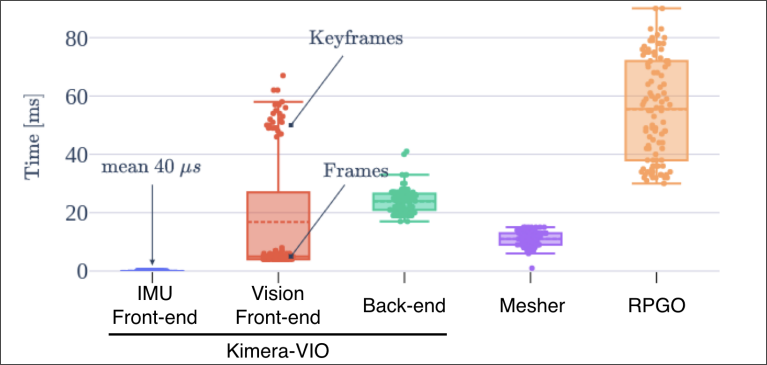
\includegraphics[width=120mm]{Timings}
  \caption{Kimera timings (see \cite{rosinol2020kimera})}\label{Fig:Timings}  
\end{figure}

\section{Conclusion}
Kimera presents a c++ Library for metric-semantic Visual-Inertial Simultaneous Localization And Mapping that is modular and able to perform in a low performance environment, allowing further research and developments in several distinct field, ranging from simultaneous localisation and mapping to semantic segmentation.
Kimeras Modules generally perform well, with the combination of Kimera-VIO and Kimera-RPGO outperforming similar state of the art libraries.
Kimera-Meshers mesh is build quickly and allows for low level navigation tasks, while Kimera-Semantics builds an accurate metric-semantic mesh.


{\small                   % use small if you need it
\bibliographystyle{plain}
\bibliography{paper}       % use a bib-file paper.bib to collect your references
}

\end{document}

